\documentclass[a4]{article}
\pagestyle{myheadings}

%%%%%%%%%%%%%%%%%%%
% Packages/Macros %
%%%%%%%%%%%%%%%%%%%
\usepackage{mathrsfs}


\usepackage{fancyhdr}
\pagestyle{fancy}
\lhead{}
\chead{}
\rhead{}
\lfoot{}
\cfoot{} 
\rfoot{\normalsize\thepage}
\renewcommand{\headrulewidth}{0pt}
\renewcommand{\footrulewidth}{0pt}
\newcommand{\RomanNumeralCaps}[1]
    {\MakeUppercase{\romannumeral #1}}

\usepackage{amssymb,latexsym}  % Standard packages
\usepackage[utf8]{inputenc}
\usepackage[russian]{babel}
\usepackage{MnSymbol}
\usepackage{mathrsfs}
\usepackage{amsmath,amsthm}
\usepackage{indentfirst}
\usepackage{graphicx}%,vmargin}
\usepackage{graphicx}
\graphicspath{{pictures/}} 
\usepackage{verbatim}
\usepackage{color}
\usepackage[nottoc,numbib]{tocbibind}
\usepackage{float}

\usepackage{listings}
\definecolor{codegreen}{rgb}{0,0.6,0}
\definecolor{codegray}{rgb}{0.5,0.5,0.5}
\definecolor{codepurple}{rgb}{0.58,0,0.82}
\definecolor{backcolour}{rgb}{0.95,0.95,0.92}
 
\lstdefinestyle{mystyle}{
    backgroundcolor=\color{backcolour},   
    commentstyle=\color{codegreen},
    keywordstyle=\color{magenta},
    numberstyle=\tiny\color{codegray},
    stringstyle=\color{codepurple},
    basicstyle=\footnotesize,
    breakatwhitespace=false,         
    breaklines=true,                 
    captionpos=b,                    
    keepspaces=true,                 
    numbers=left,                    
    numbersep=5pt,                  
    showspaces=false,                
    showstringspaces=false,
    showtabs=false,                  
    tabsize=2
}
 
\lstset{style=mystyle}

\usepackage{url}
\urldef\myurl\url{foo%.com}





\DeclareGraphicsExtensions{.pdf,.png,.jpg}% -- настройка картинок

\usepackage{epigraph} %%% to make inspirational quotes.
\usepackage[all]{xy} %for XyPic'a
\usepackage{color} 
\usepackage{amscd} %для коммутативных диграмм
%\usepackage[colorlinks,urlcolor=red]{hyperref}

%\renewcommand{\baselinestretch}{1.5}
%\sloppy
%\usepackage{listings}
%\lstset{numbers=left}
%\setmarginsrb{2cm}{1.5cm}{1cm}{1.5cm}{0pt}{0mm}{0pt}{13mm}


\newtheorem{Lemma}{Лемма}[section]
\newtheorem{Proposition}{Предложение}[section]
\newtheorem{Theorem}{Теорема}[section]
\newtheorem{Corollary}{Следствие}[section]
\newtheorem{Remark}{Замечание}[section]
\newtheorem{Definition}{Определение}[section]
\newtheorem{Designations}{Обозначение}[section]




%%%%%%%%%%%%%%%%%%%%%%% 
%Подготовка оглавления% 
%%%%%%%%%%%%%%%%%%%%%%% 
\usepackage[titles]{tocloft}
\renewcommand{\cftdotsep}{2} %частота точек
\renewcommand\cftsecleader{\cftdotfill{\cftdotsep}}
\renewcommand{\cfttoctitlefont}{\hspace{0.38\textwidth} \LARGE\bfseries} 
\renewcommand{\cftsecaftersnum}{.}
\renewcommand{\cftsubsecaftersnum}{.}
\renewcommand{\cftbeforetoctitleskip}{-1em} 
\renewcommand{\cftaftertoctitle}{\mbox{}\hfill \\ \mbox{}\hfill{\footnotesize Стр.}\vspace{-0.5em}} 
%\renewcommand{\cftchapfont}{\normalsize\bfseries \MakeUppercase{\chaptername} } 
%\renewcommand{\cftsecfont}{\hspace{1pt}} 
\renewcommand{\cftsubsecfont}{\hspace{1pt}} 
%\renewcommand{\cftbeforechapskip}{1em} 
\renewcommand{\cftparskip}{3mm} %определяет величину отступа в оглавлении
\setcounter{tocdepth}{5} 
\renewcommand{\listoffigures}{\begingroup %добавляем номер в список иллюстраций
\tocsection
\tocfile{\listfigurename}{lof}
\endgroup}
\renewcommand{\listoftables}{\begingroup %добавляем номер в список иллюстраций
\tocsection
\tocfile{\listtablename}{lot}
\endgroup}


   
   
%\renewcommand{\thelikesection}{(\roman{likesection})}
%%%%%%%%%%%
% Margins %
%%%%%%%%%%%
\addtolength{\textwidth}{0.7in}
\textheight=630pt
\addtolength{\evensidemargin}{-0.4in}
\addtolength{\oddsidemargin}{-0.4in}
\addtolength{\topmargin}{-0.4in}

%%%%%%%%%%%%%%%%%%%%%%%%%%%%%%%%%%%
%%%%%%Переопределение chapter%%%%%% 
%%%%%%%%%%%%%%%%%%%%%%%%%%%%%%%%%%%
\newcommand{\empline}{\mbox{}\newline} 
\newcommand{\likechapterheading}[1]{ 
\begin{center} 
\textbf{\MakeUppercase{#1}} 
\end{center} 
\empline} 

%%%%%%%Запиливание переопределённого chapter в оглавление%%%%%% 
\makeatletter 
\renewcommand{\@dotsep}{2} 
\newcommand{\l@likechapter}[2]{{\bfseries\@dottedtocline{0}{0pt}{0pt}{#1}{#2}}} 
\makeatother 
\newcommand{\likechapter}[1]{ 
\likechapterheading{#1} 
\addcontentsline{toc}{likechapter}{\MakeUppercase{#1}}} 




\usepackage{xcolor}
\usepackage{hyperref}
\definecolor{linkcolor}{HTML}{000000} % цвет ссылок
\definecolor{urlcolor}{HTML}{AA1622} % цвет гиперссылок
 
\hypersetup{pdfstartview=FitH,  linkcolor=linkcolor,urlcolor=urlcolor, colorlinks=true}

%%%%%%%%%%%%
% Document %
%%%%%%%%%%%%

%%%%%%%%%%%%%%%%%%%%%%%%%%%%%
%%%%%%главы -- section*%%%%%%
%%%%section -- subsection%%%%
%subsection -- subsubsection%
%%%%%%%%%%%%%%%%%%%%%%%%%%%%%
\def \newstr {\medskip \par \noindent} 



\begin{document}
\def\contentsname{\LARGE{Содержание}}
\thispagestyle{empty}
\begin{center} 
\vspace{2cm} 
{\Large \sc Санкт-Петербургский Политехнический}\\
\vspace{2mm}
{\Large \sc Университет} им. {\Large\sc Петра Великого}\\
\vspace{1cm}
{\large \sc Институт прикладной математики и механики\\ 
\vspace{0.5mm}
\textsc{}}\\ 
\vspace{0.5mm}
{\large\sc Кафедра прикладной математики}\\
\vspace{15mm}
%\rule[0.5ex]{\linewidth}{2pt}\vspace*{-\baselineskip}\vspace*{3.2pt} 
%\rule[0.5ex]{\linewidth}{1pt}\\[\baselineskip] 
{\huge \sc Отчёт по лабораторным работам №$1-4$\\
\vspace{4mm}
Исследование распределений
\vspace{6mm}
 }
\vspace*{2mm}
%\rule[0.7ex]{\linewidth}{1pt}\vspace*{-\baselineskip}\vspace{3.2pt} 
%\rule[0.5ex]{\linewidth}{2pt}\\ 
\vspace{1cm}

{\sc $3$ курс$,$ группа $33631/2$}

\vspace{2cm} 
Студент \hfill Д. А. Плаксин\\
\vspace{1cm}
Преподаватель \hfill Баженов А. Н.\\
\vspace{20mm} 

\end{center} 
%\author{Я}
\begin{center}
\vfill {\large\textsc{Санкт-Петербург}}\\ 
2019 г.
\end{center}

%%%%%%%%%%%%%%%%%%%%%%%%%%%%%%%%%%%%%%%%%%%%%%%%%%%%%%%%%%%%%%%%%%%%%%%%%%%%%%%%%%%%%%%%%%%%%%
%\ \\[4cm]

%\rm
%%%%%%%%%%%%%%%%%%%%%%%%%%%%%%%%%%%%%%%%%%%%%%%%%%%%%%%%%%%%%%%%%%%%%%%%%%%%%%%%%%%%%%%%%%%%%%
\newpage
\pagestyle{plain}

%\begin{center}
%\begin{abstract} 

%\end{abstract}

%\end{center}

\newpage
\tableofcontents{}
\newpage
\listoffigures{}
\listoftables{}
\newpage

\section{Постановка задачи}
В данных работах надо было сгенерировать выборки разных мощностей для пяти распределений:
Распределения \cite{distr_formulas}:
\begin{enumerate}
\item Стандартное нормальное распределение
\item Стандартное распределение Коши
\item Распределение Лапласа с коэффициентом масштаба $\sqrt{2}$ и нулевым коэффициентом сдвига.
\item Равномерное распределение на отрезке $\left[-\sqrt{3}, \sqrt{3}\right]$
\item Распределение Пуассона со значением матожидания равным двум.
\end{enumerate}

Для этих выборок надо было:
\begin{enumerate}
    \item Построить гистограммы и графики плотности распределения.
    \item Вычислить характеристики положения. Вычисления необходимо повторить $1000$ раз для каждой выборки, найти среднее характеристик положения и их квадратов, вычислить оценку дисперсии, полученные данные представить в виде таблиц.
    \item Построить боксплот Тьюки, затем для каждого распределения определить процент выбросов (вычислив средний процент выбросов из $1000$ экспериментов) и сравнить полученные результаты с теоретическими.
    \item Построить эмпирические функции распределения и ядерные оценки плотности распределения на отрезке $[-4;4].$	
\end{enumerate}



\section{Теория}
\subsection{Плотности распределения вероятностей}

Плотностью распределения вероятностей непрерывной случайной величины называется первая производная от функции распределения. Смысл плотности распределения в том, что она показывает, как часто появляется случайная величина в некоторой окрестности точки при повторении опытов.

Для рассматриваемых в этой работе пяти распределений известны плотности их вероятности:

\begin{equation}\label{eqn:normal}
\text{Нормальное распределение } N(x,0,1) = \frac{1}{\sqrt{2\pi}}e^{-\frac{x^2}{2}}
\end{equation} 

\begin{equation}\label{eqn:cauchy}
\text{Распределение Коши } C(x,0,1) = \frac{1}{\pi(1+x^2)}
 \end{equation}
 
 \begin{equation}\label{eqn:laplace}
\text{Распределение Лапласа } L\left( x,0,\frac{1}{\sqrt{2}}\right) = \frac{1}{\sqrt{2}}e^{-\sqrt{2}\vert x\vert}
 \end{equation}
 
 \begin{equation}\label{eqn:poisson}
\text{Распределение Пуассона } P(\lambda,k) = \frac{\lambda^k}{k!}e^{-\lambda}
\end{equation}  

\begin{equation}\label{eqn:uniform}
\text{Равномерное распределение } M(x,-\sqrt{3}, \sqrt{3}) = 
 \begin{cases}
   \frac{1}{2\sqrt{3}} &\vert x\vert \leqslant \sqrt{3}\\
   0 &\vert x\vert > \sqrt{3}
 \end{cases}
\end{equation}

\subsection{Характеристики положения}
Характеристики положения дают информацию о расположении значений выборки на числовой прямой и характеризуют этот признак с точки зрения некоторого среднего значения.

Для рассматриваемых в этой работе характеристик положения данных известны формулы для их вычисления:

\begin{enumerate}
\item Выборочное среднее \cite{average}:
\begin{equation}\label{eqn:average}
\overline{x} = \frac{1}{n}\sum_{i=1}^n x_i \hfill  
\end{equation}
\item Выборочная медиана \cite{med}:
\begin{equation}
med\; x = \begin{cases}
x_{k+1}, & n = 2k+1\\
\frac{1}{2}\left(x_k+x_{k+1}\right), & n = 2k
\end{cases} \hfill  \label{eqn:med}
\end{equation}
\item Полусумма экстремальных значений \cite{mean_extr}:
\begin{equation}
Z_R = \frac{1}{2}\left(x_1+x_n\right) \hfill  \label{eqn:mean_extr}
\end{equation}
\item Полусумма квартилей \cite{quartiles}:
\begin{equation}
Z_Q = \frac{1}{2}\left(Z_{\frac{1}{4}}+Z_{\frac{3}{4}}\right) \hfill  \label{eqn:quartiles}
\end{equation}
\item Усечённое среднее \cite{cut_mean}:
\begin{equation}
Z_{tr} = \frac{1}{n - 2r}\sum_{i=r+1}^{n-r} x_i \hfill  \label{eqn:cut_mean}
\end{equation}
\end{enumerate}


\subsection{Боксплот Тьюки}

Боксплот Тьюки - график, использующийся в описательной статистике, изображающий одномерное распределение вероятностей.

Такой вид диаграммы в удобной форме показывает медиану, нижний и верхний квартили, минимальное и максимальное значение выборки и выбросы.

Выбросом в статистике называют результат измерения, выделяющийся из общей выборки.

\subsection{Эмпирические функции и ядерные оценки}

Эмпирическая функция распределения \cite{emp}, построенная по выборке $X = \left(X_1,\ldots, X_n\right)$ есть случайная функция $F_n(y),$ определённая на $\mathbb{R}:$
\begin{equation}
F_n(y) = \sum\limits_{i=1}^n I\left(X_i < y\right) \;\;\text{где}\; I\left(X_i < y\right) = \begin{cases} 
1, & X_i < y\\
0, & \text{иначе}
\end{cases}\hfill\label{eqn:emp}
\end{equation}


$X = \left(X_1,\ldots, X_n\right)$ есть одномерная выборка одинаково распределённых элементов, с плотностью распределения $f.$

Ядерная оценка плотности \cite{art}:
\begin{equation}
    f_h(x) = \frac{1}{nh}\sum\limits_{i=1}^nK\left(\frac{x-x_i}{h}\right)\label{eqn:art}
\end{equation}
где $K$ является ядром, а $h>0$ является сглаживающим параметром, и называется шириной полосы.

В данной работе в качестве ядра была выбрана плотность вероятности стандартного нормального распределения \cite{link:pdf}:

\begin{equation}
    K(x) = \frac{1}{\sqrt{2\pi}}e^{-\frac{x^2}{2}}
\end{equation}

\section{Реализация}
Для генерации выборки был использован $Python\;3.7$: модуль $random$ библиотеки $numpy$ \cite{numpy} для генерации случайных чисел с различными распределениями. 

Обработка функций распределений была сделана с помощью модуля $scipy$ \cite{skp}.


После вычисления характеристик положения $1000$ раз среднее значение и дисперсия находились по следующей формуле: 
\begin{equation}
D(z) = E\left(z^2\right) - E^2(z),\; \text{где}\; E(z) = \frac{1}{n}\sum_{i=1}^n z_i
\end{equation}


Боксплот Тьюки был построен средствами библиотеки matplotlib \cite{plotlib}.

Правая и левые границы:  $R- LQ - l(UQ - LQ),\;L = UQ -k(UQ - LQ),$ где $k$ обычно полагают равным $1.5$ \cite{sas}

Число выбросов определялось таким образом: если значение из выборки находится вне установленных левой и правых границ, то оно является выбросом.



\newpage
\section{Результаты}


\subsection{Плотности распределения вероятностей}

\begin{figure}[H]
    \centering
    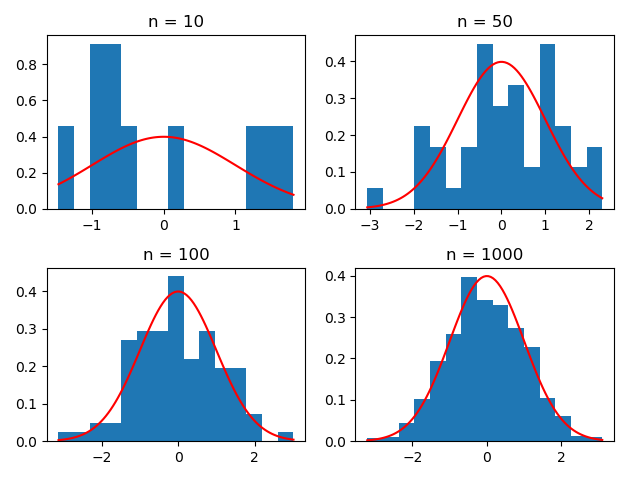
\includegraphics[width=\textwidth]{distribution_normal.png} 
    \caption{Нормальное распределение \eqref{eqn:normal}}
    \label{fig:dis_norm_gis}
\end{figure}

\begin{figure}[H]
    \centering
    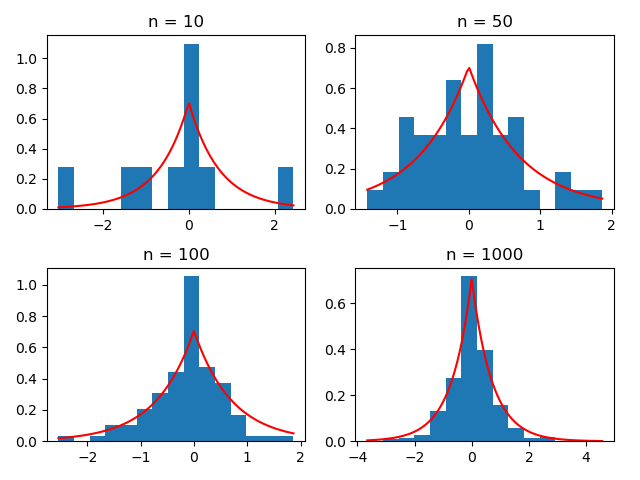
\includegraphics[width=\textwidth]{distribution_laplace.png}
    \caption{Распределение Лапласа \eqref{eqn:laplace}}
    \label{fig:dis_lapl_gis}
\end{figure}

\begin{figure}[H]
    \centering
    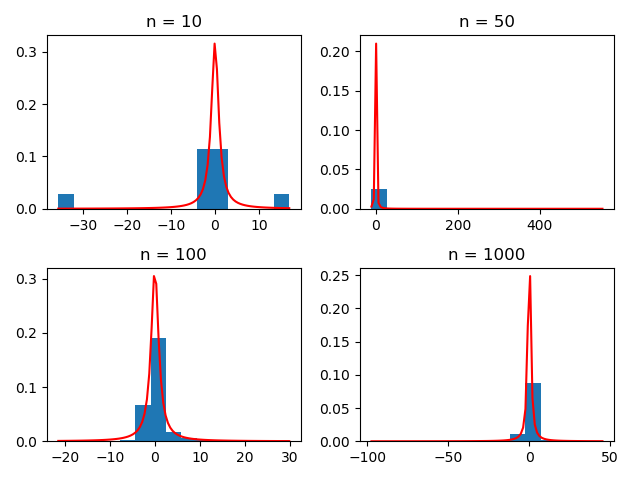
\includegraphics[width=\textwidth]{distribution_cauchy2.png}
    \caption{Распределение Коши \eqref{eqn:cauchy}}
    \label{fig:dis_cauc_gis}
\end{figure}

\begin{figure}[H]
    \centering
    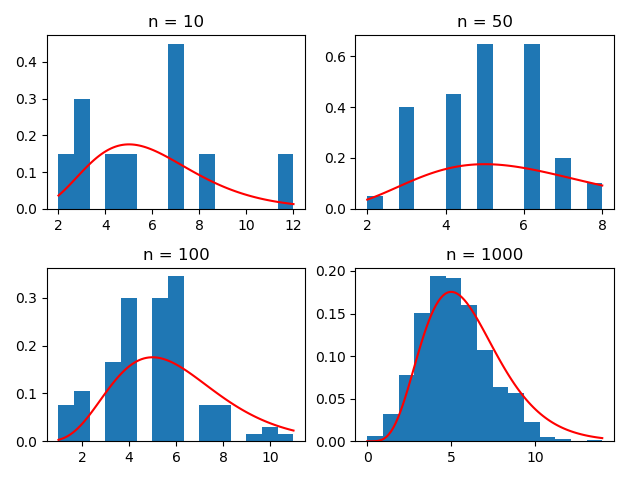
\includegraphics[width=\textwidth]{distribution_poisson.png}
    \caption{Распределение Пуассона \eqref{eqn:poisson}}
    \label{fig:dis_pois_gis}
\end{figure}

\begin{figure}[H]
    \centering
    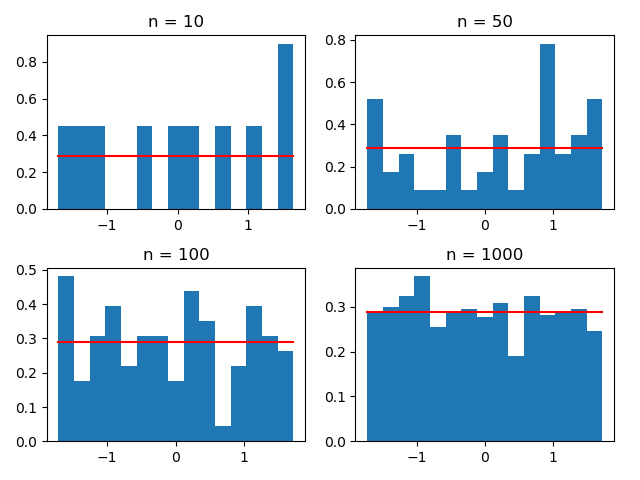
\includegraphics[width=\textwidth]{distribution_uniform.png}
    \caption{Равномерное распределение \eqref{eqn:uniform}}
    \label{fig:dis_uni_gis}
\end{figure}


\subsection{Характеристики положения}
\begin{table}[H]
\caption{\label{tab:normal} Стандартное нормальное распределение \eqref{eqn:normal}.}
\begin{center}
\begin{tabular}{|c|c|c|c|c|c|}
\hline
$n = 20$ & average & med & $Z_R$ & $Z_Q$ & $Z_{tr},\;r=\frac{n}{4}$\\
\hline
$E =$ & $-0.00$ & $-0.00$ & $0.0$ & $0.00$ & $-0.01$\\
\hline
$D =$ & $0.051763$ & $0.072023$ & $0.149073$ & $0.058764$ & $0.059323$\\
\hline
$n = 60$ & average & med & $Z_R$ & $Z_Q$ & $Z_{tr},\;r=\frac{n}{4}$\\
\hline
$E =$ & $0.00$ & $0.00$ & $-0.0$ & $-0.00$ & $-0.00$\\
\hline
$D =$ & $0.016322$ & $0.026125$ & $0.110309$ & $0.020489$ & $0.020389$\\
\hline
$n = 100$ & average & med & $Z_R$ & $Z_Q$ & $Z_{tr},\;r=\frac{n}{4}$\\
\hline
$E =$ & $0.000$ & $-0.00$ & $-0.00$ & $-0.00$ & $-0.00$\\
\hline
$D =$ & $0.009563$ & $0.015479$ & $0.096256$ & $0.012569$ & $0.012224$\\
\hline
\end{tabular}
\end{center}
\end{table}

\begin{table}[H]
\caption{\label{tab:cauchy} Стандартное распределение Коши \eqref{eqn:cauchy}.}
\begin{center}
\begin{tabular}{|c|c|c|c|c|c|}
\hline
$n = 20$   & average & med & $Z_R$ & $Z_Q$ & $Z_{tr},\;r=\frac{n}{4}$\\ \hline
$E =$      & 	$3.414266$    &	$-0.012522$   &	$-5.262327$   &	$-0.027313$   &	$0.020763$\\ \hline
$D =$       &	$12977.113689$ &	$0.130212$   & 	$12626.531931$ &	$0.371684$    &	$0.150542$\\    \hline
					
$n = 60$   & average & med & $Z_R$ & $Z_Q$ & $Z_{tr},\;r=\frac{n}{4}$\\ \hline
$E =$   &    	$-1.180135$   &	$-0.008143$   &	$-69.304468$  &	$0.007723$ &   	$-0.006201$\\   \hline
$D =$      & 	$1424.446598$ &	$0.038886$   & 	$6240734.028690$ &	$0.086309$ &   	$0.042207$\\   \hline 
					
$n = 100$   & average & med & $Z_R$ & $Z_Q$ & $Z_{tr},\;r=\frac{n}{4}$\\ \hline
$E =$      & 	$0.811064$    &	$-0.003271$   &	$30.434787$  & 	$0.002690$  &  	$-0.008544 $\\  \hline
$D =$    &  	$350.070803$  &	$0.023004$    &	$1465401.042218$ &	$0.054476$ &   	$0.025649$\\    
\hline
\end{tabular}
\end{center}
\end{table}

\begin{table}[H]
\caption{\label{tab:laplace} Распределение Лапласа \eqref{eqn:laplace}.}
\begin{center}
\begin{tabular}{|c|c|c|c|c|c|}
\hline
$n = 20$    & average & med & $Z_R$ & $Z_Q$ & $Z_{tr},\;r=\frac{n}{4}$\\ \hline 
$E = $    &  	$-0.01$  & 	$-0.01$   &	$-0.0$   &	$0.00$    &	$-0.00$   \\ \hline
$D = $     & 	$0.047943$  &  	$0.031492$    &	$0.436478$    &	$0.047849$    &	$0.031600$    \\ \hline
					
$n = 60$  & average & med & $Z_R$ & $Z_Q$ & $Z_{tr},\;r=\frac{n}{4}$\\ \hline
$E = $     & 	$0.00$    &	$-0.00$   &	$-0.0$   &	$-0.00$   &	$-0.00$   \\ \hline
$D =$      & 	$0.017707$   & 	$0.010050$   & 	$0.455793$    &	$0.014958$    &	$0.010114$    \\ \hline
					
$n = 100$   & average & med & $Z_R$ & $Z_Q$ & $Z_{tr},\;r=\frac{n}{4}$\\ \hline
$E =$      & 	$0.005$    &	$0.004$    &	$0.0$    &	$0.00$    &	$-0.000$   \\ \hline
$D = $     & 	$0.009733$    &	$0.006307$   & 	$0.409248$  &  	$0.010233$    &	$0.006262$    \\ 
\hline
\end{tabular}
\end{center}
\end{table}

\begin{table}[H]
\caption{\label{tab:uniform} Равномерное распределение \eqref{eqn:uniform}.}
\begin{center}
\begin{tabular}{|c|c|c|c|c|c|}
\hline
$n = 20$  & average & med & $Z_R$ & $Z_Q$ & $Z_{tr},\;r=\frac{n}{4}$\\ \hline
$E =$       &	$-0.00$  & 	$-0.0$  & 	$0.00$    &	$-0.00$   &	$0.00$  \\ \hline  
$D =$       &	$0.046929$    &	$0.126544$    &	$0.013805$    &	$0.070389$   & 	$0.098176$    \\ \hline
					
$n = 60$  & average & med & $Z_R$ & $Z_Q$ & $Z_{tr},\;r=\frac{n}{4}$\\ \hline
$E =$       &	$0.00$   & 	$-0.00$   &	$-0.000$   &	$0.00$   & 	$0.00$    \\ \hline
$D =$       &	$0.018149$    &	$0.048531$   & 	$0.001583$    &	$0.023893$   & 	$0.032310$    \\ \hline
					
$n = 100$  & average & med & $Z_R$ & $Z_Q$ & $Z_{tr},\;r=\frac{n}{4}$\\ \hline
$E =$     &  	$0.00$    &	$0.00$    &	$0.0010 $  & 	$0.00$   & 	$0.00$    \\ \hline
$D =$    &   	$0.010555$    &	$0.029134$    &	$0.000562$   & 	$0.014285$   & 	$0.020388$    \\
\hline
\end{tabular}
\end{center}
\end{table}

\begin{table}[H]
\caption{\label{tab:poisson} Распределение Пуассона \eqref{eqn:poisson}.}
\begin{center}
\begin{tabular}{|c|c|c|c|c|c|}
\hline
$n = 20$   & average & med & $Z_R$ & $Z_Q$ & $Z_{tr},\;r=\frac{n}{4}$\\ \hline
$E =$     &  	$1.99$    &	$1.8$  &  	$2.5$   & 	$1.9$  &  	$1.8$    \\ \hline
$D =$     &  	$0.096696$    &	$0.201928$    &	$0.325744$   & 	$0.126251$  &  	$0.125845$    \\ \hline
					
$n = 60$   & average & med & $Z_R$ & $Z_Q$ & $Z_{tr},\;r=\frac{n}{4}$\\ \hline
$E =$      & 	$1.99$    &	$1.92$    &	$2.9$   & 	$1.94$    &	$1.84$    \\ \hline
$D =$       &	$0.032178$    &	$0.063700$   & 	$0.245694$   & 	$0.033469$   & 	$0.046742$    \\ \hline
					
$n = 100$   & average & med & $Z_R$ & $Z_Q$ & $Z_{tr},\;r=\frac{n}{4}$\\ \hline
$E =$      & 	$1.99$    &	$1.96$    &	$3.1$  &  	$1.96$   & 	$1.83$    \\ \hline
$D =$      & 	$0.020435$    &	$0.030204$   & 	$0.239758$   & 	$0.018016$  &  	$0.026728$    \\
\hline
\end{tabular}
\end{center}
\end{table}


\subsection{Боксплот Тьюки}
\begin{center}

\begin{figure}[H]
\caption{Boxplot нормальное распределение \eqref{eqn:normal}}
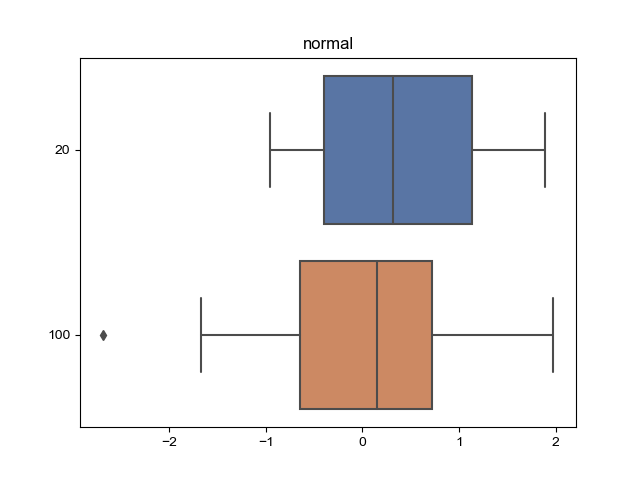
\includegraphics[width=\textwidth]{normal.png}
\end{figure}

\begin{figure}[H]
\caption{Boxplot стандартное распределение Лапласа \eqref{eqn:laplace}}
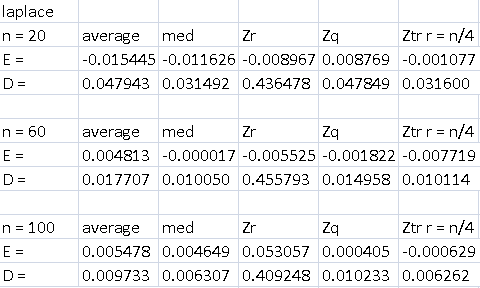
\includegraphics[width=\textwidth]{laplace.png} 
\end{figure}

\begin{figure}[H]
\caption{Boxplot стандартное распределение Коши \eqref{eqn:cauchy}}
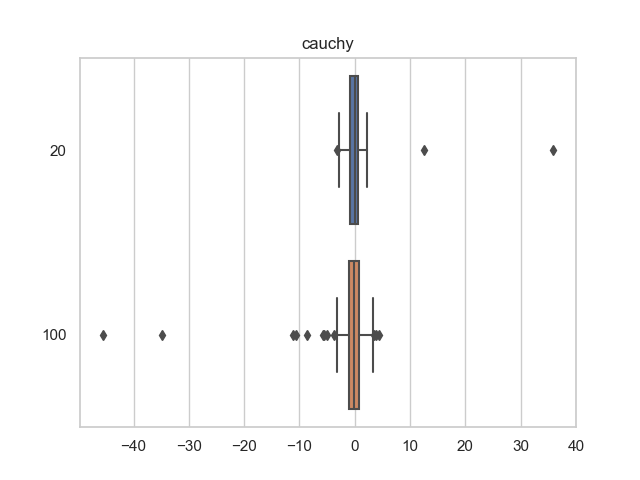
\includegraphics[width=\textwidth]{cauchy.png} 
\end{figure}

\begin{figure}[H]
\caption{Boxplot распределение Пуассона \eqref{eqn:poisson}}
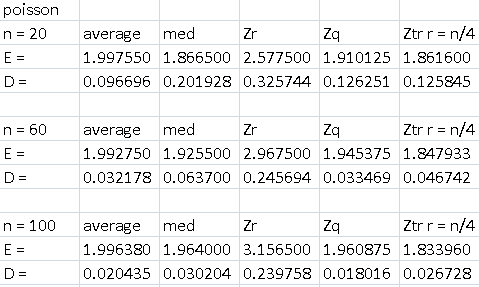
\includegraphics[width=\textwidth]{poisson.png} 
\end{figure}

\begin{figure}[H]
 \caption{Boxplot равномерное распределение \eqref{eqn:uniform}}
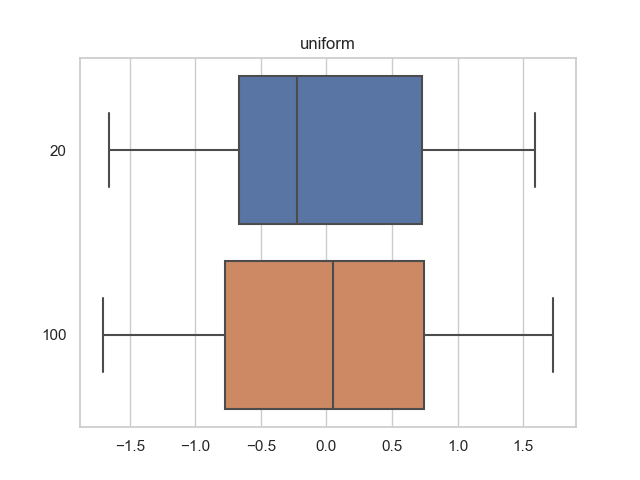
\includegraphics[width=\textwidth]{uniform.png}
\end{figure}

\begin{table}[H]
    
    \caption{Зависимость выбросов от размера выборки}
    \label{tab:my_label}
    \begin{center}
    \vspace{5mm}
    \begin{tabular}{|c|c|}
    \hline
    Выборка & Процент выбросов\\
    \hline
         normal	&\\
         \hline
n = 20   & 	2    \\
\hline
n = 100   &	1    \\
	\hline
cauchy	&\\
\hline
n = 20   & 	15    \\
\hline
n = 100  & 	16    \\
	\hline
laplace	&\\
\hline
n = 20    &	7    \\
\hline
n = 100   &	6    \\
	\hline
uniform	&\\
\hline
n = 20    &	0    \\
\hline
n = 100   &	0   \\ 
	\hline
poisson	&\\
\hline
n = 20   & 	3    \\
\hline
n = 100  & 	0    \\
\hline
    \end{tabular}
    
    \end{center}
    
\end{table}

\end{center}








\subsection{Ядерная оценка плотности}
\begin{center}

\begin{figure}[H]
\caption{Эмпирическая функция для нормального стандартного распределения \eqref{eqn:normal}}
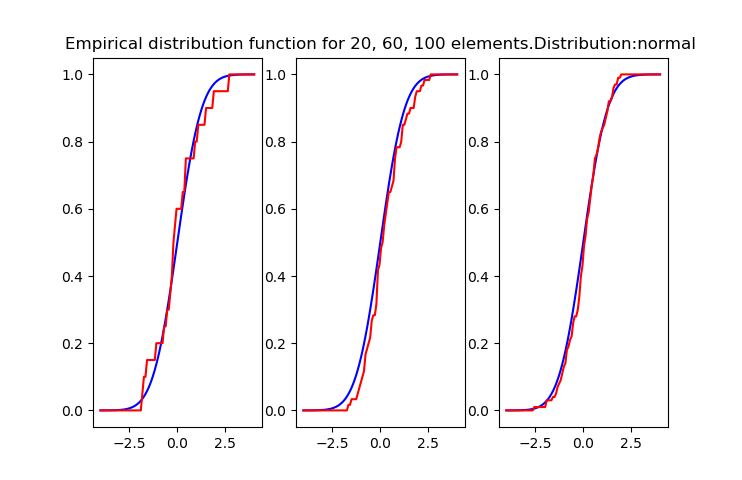
\includegraphics[width=\textwidth]{e_normal.png}
\end{figure}

\begin{figure}[H]
\caption{Эмпирическая функция для стандартного распределения Лапласа \eqref{eqn:laplace}}
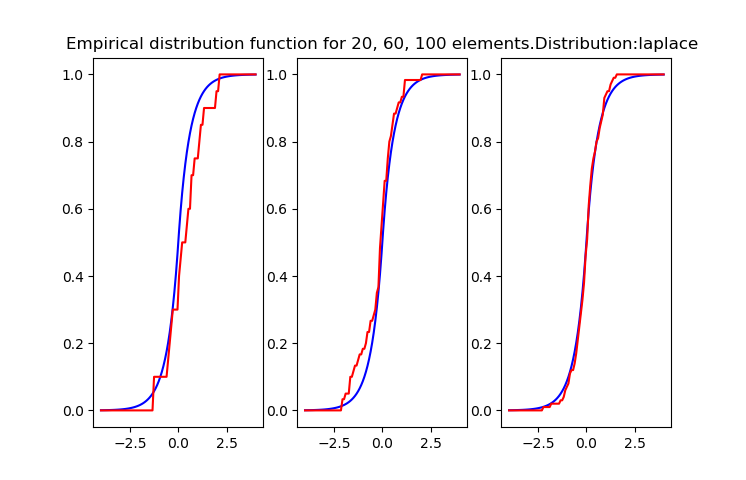
\includegraphics[width=\textwidth]{e_laplace.png} 
\end{figure}

\begin{figure}[H]
\caption{Эмпирическая функция для стандартного распределения Коши \eqref{eqn:cauchy}}
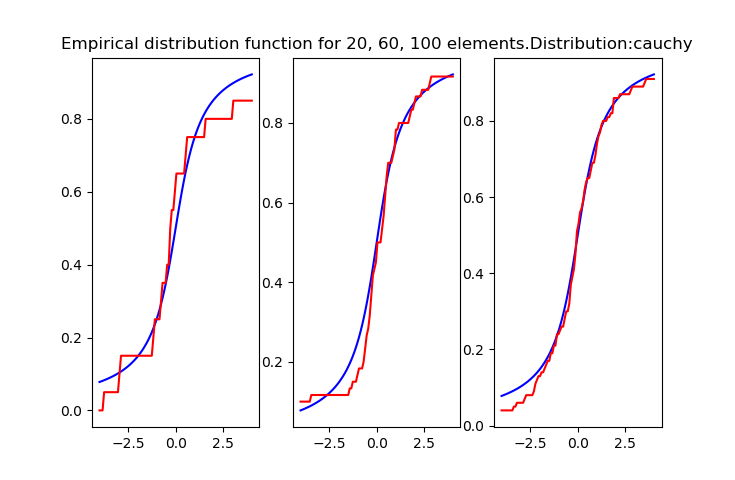
\includegraphics[width=\textwidth]{e_cauchy.png} 
\end{figure}

\begin{figure}[H]
\caption{Эмпирическая функция для распределения Пуассона \eqref{eqn:poisson}}
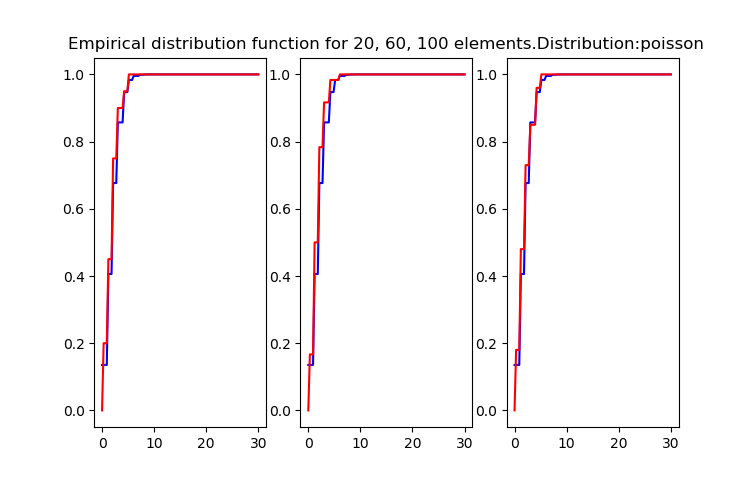
\includegraphics[width=\textwidth]{e_poisson.png} 
\end{figure}

\begin{figure}[H]
 \caption{Эмпирическая функция для равномерного распределения \eqref{eqn:uniform}}
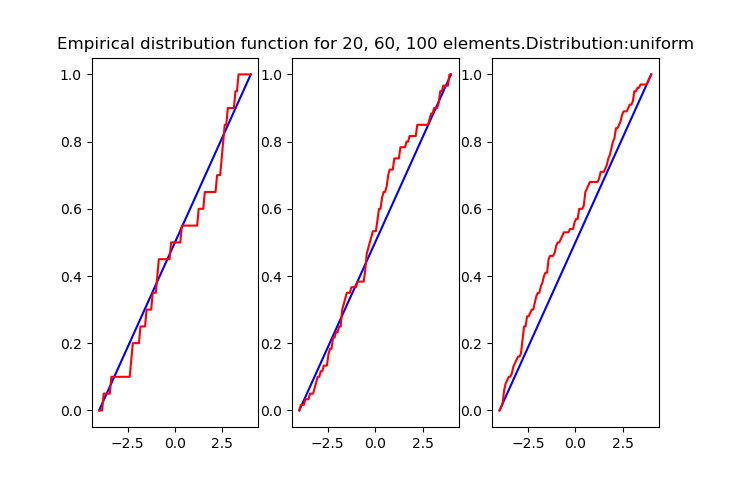
\includegraphics[width=\textwidth]{e_uniform.png}
\end{figure}
\end{center}
\subsection{Эмпирические функции и ядерные оценки}

\begin{center}
    \begin{figure}[H]
 \caption{Ядерная функция плотности для нормального распределения \eqref{eqn:normal}, n = 20}
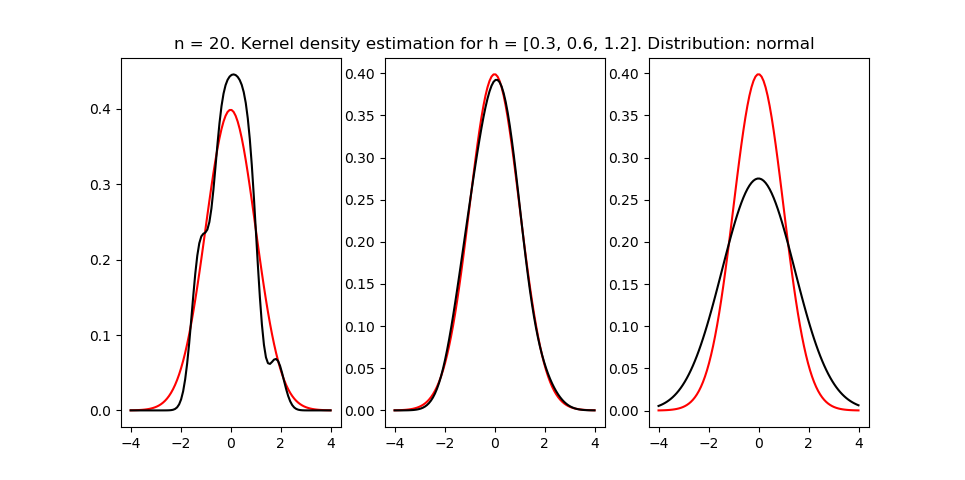
\includegraphics[width=\textwidth]{d_normal20.png}
\end{figure}
    \begin{figure}[H]
 \caption{Ядерная функция плотности для нормального распределения \eqref{eqn:normal}, n = 60}
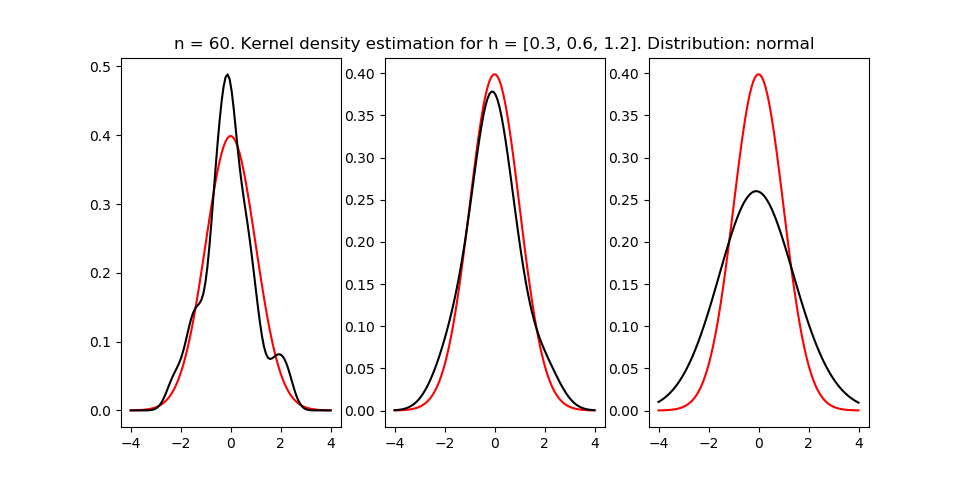
\includegraphics[width=\textwidth]{d_normal60.png}
\end{figure}
    \begin{figure}[H]
 \caption{Ядерная функция плотности для нормального распределения \eqref{eqn:normal}, n = 100}
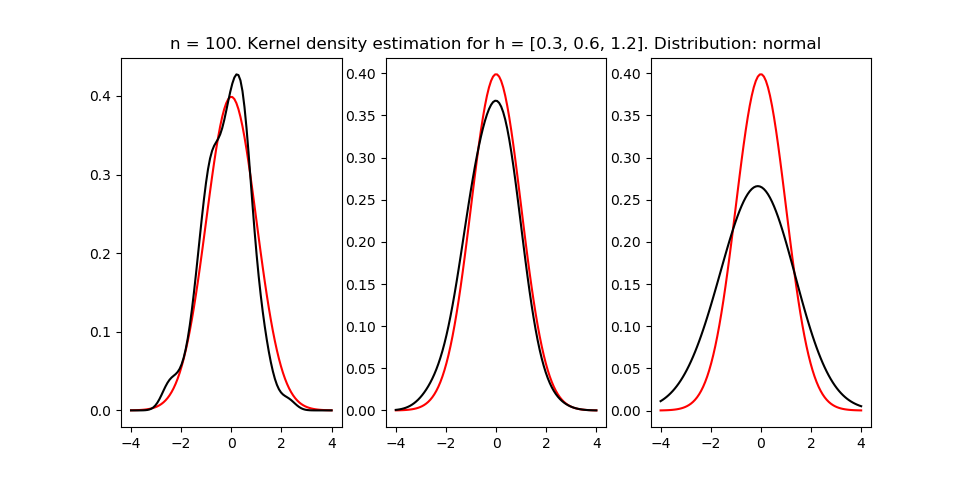
\includegraphics[width=\textwidth]{d_normal100.png}
\end{figure}

    \begin{figure}[H]
 \caption{Ядерная функция плотности для распределения Лапласа \eqref{eqn:laplace}, n = 20}
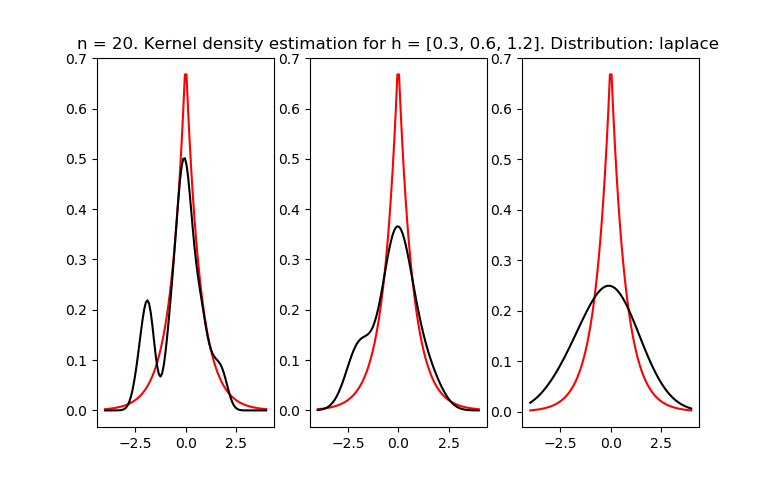
\includegraphics[width=\textwidth]{d_laplace20.png}
\end{figure}
    \begin{figure}[H]
 \caption{Ядерная функция плотности для распределения Лапласа \eqref{eqn:laplace}, n = 60}
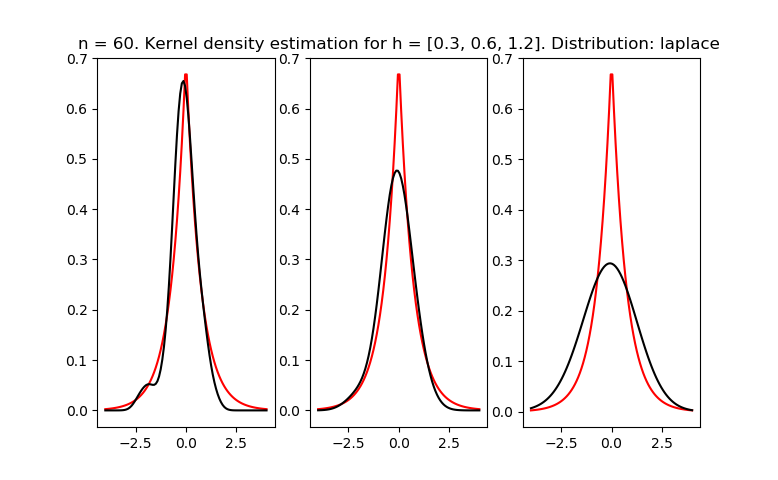
\includegraphics[width=\textwidth]{d_laplace60.png}
\end{figure}
    \begin{figure}[H]
 \caption{Ядерная функция плотности для распределения Лапласа \eqref{eqn:laplace}, n = 100}
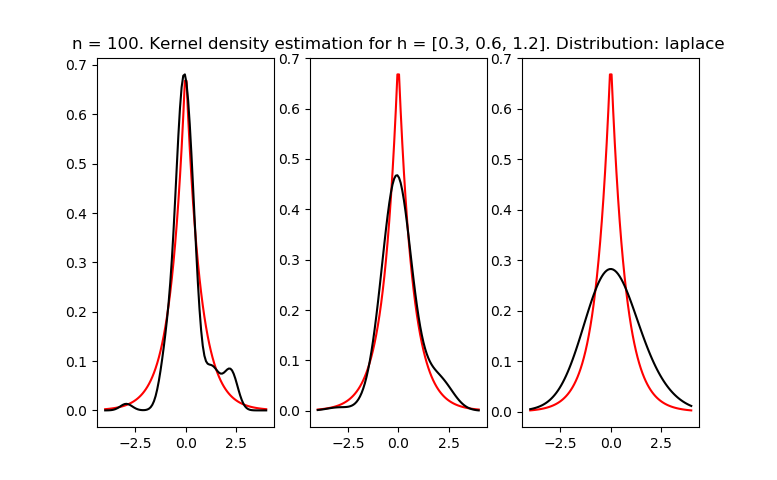
\includegraphics[width=\textwidth]{d_laplace100.png}
\end{figure}

    \begin{figure}[H]
 \caption{Ядерная функция плотности для распределения Коши \eqref{eqn:cauchy}, n = 20}
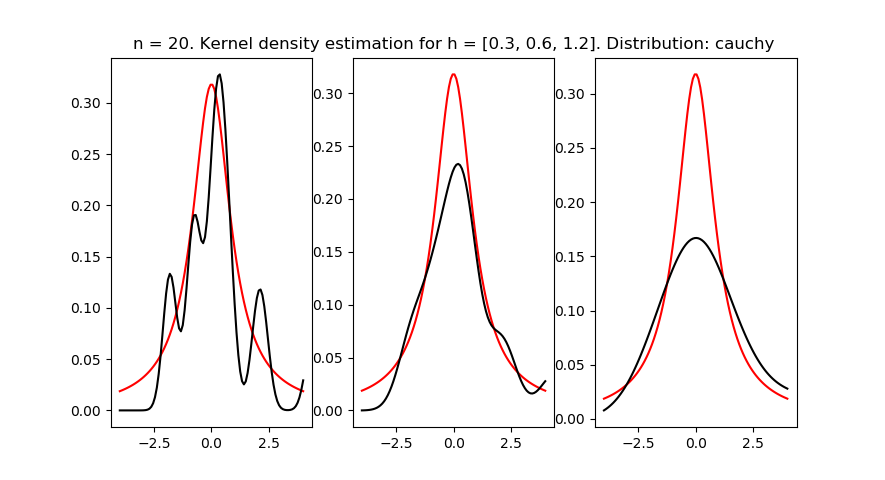
\includegraphics[width=\textwidth]{d_cauchy20.png}
\end{figure}
    \begin{figure}[H]
 \caption{Ядерная функция плотности для распределения Коши \eqref{eqn:cauchy} 60}
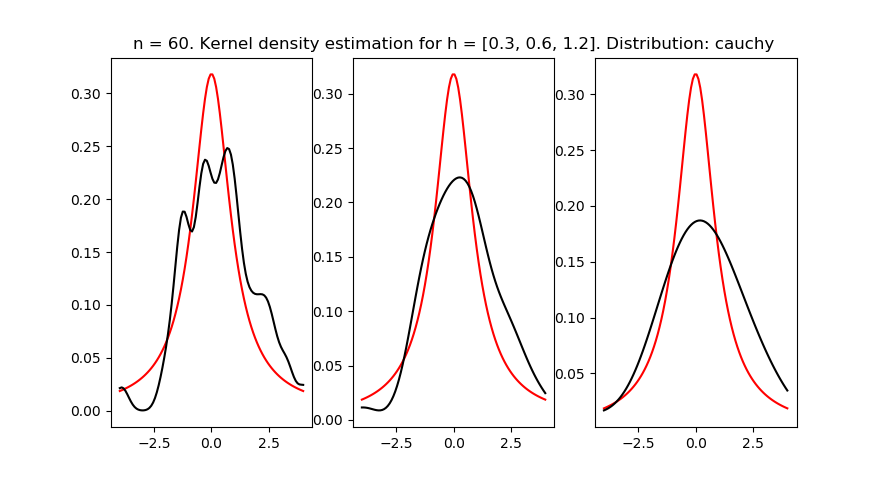
\includegraphics[width=\textwidth]{d_cauchy60.png}
\end{figure}
    \begin{figure}[H]
 \caption{Ядерная функция плотности для распределения Коши \eqref{eqn:cauchy}, n = 100}
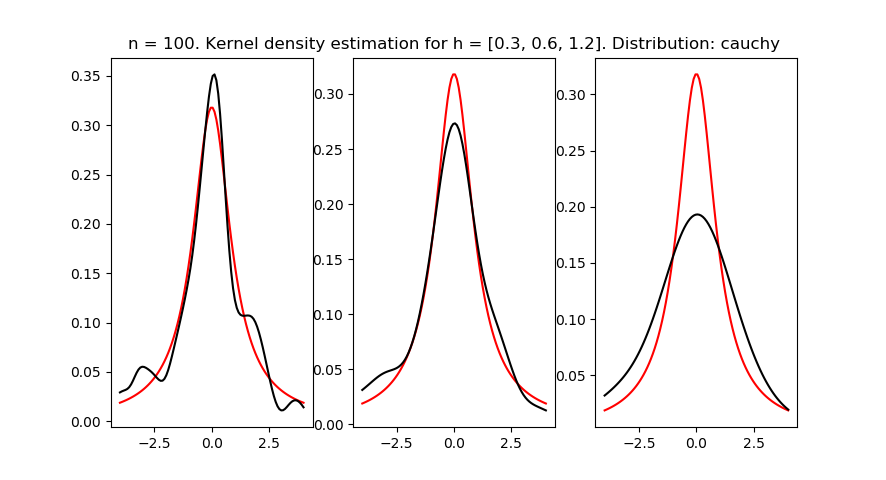
\includegraphics[width=\textwidth]{d_cauchy100.png}
\end{figure}

    \begin{figure}[H]
 \caption{Ядерная функция плотности для распределения Пуассона \eqref{eqn:poisson}, n = 20}
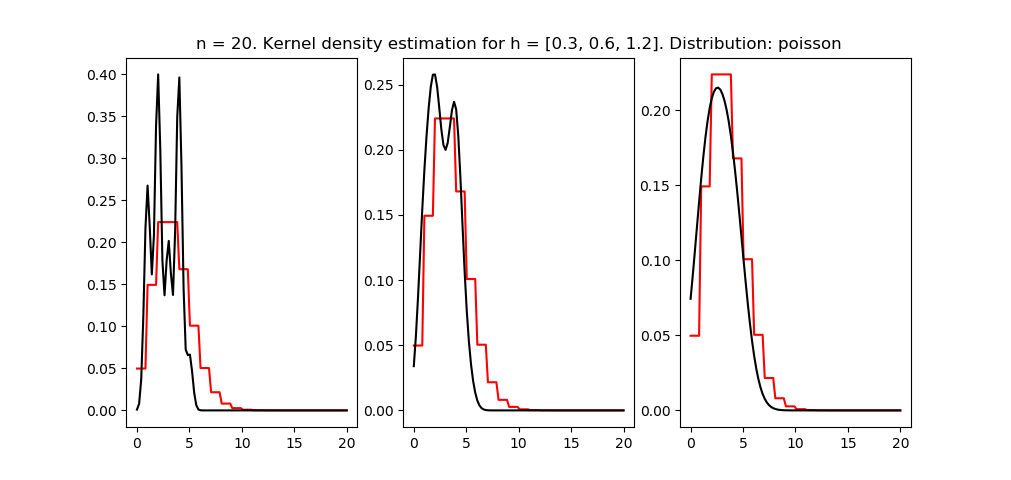
\includegraphics[width=\textwidth]{d_poisson20.png}
\end{figure}
    \begin{figure}[H]
 \caption{Ядерная функция плотности для распределения Пуассона \eqref{eqn:poisson}, n = 60}
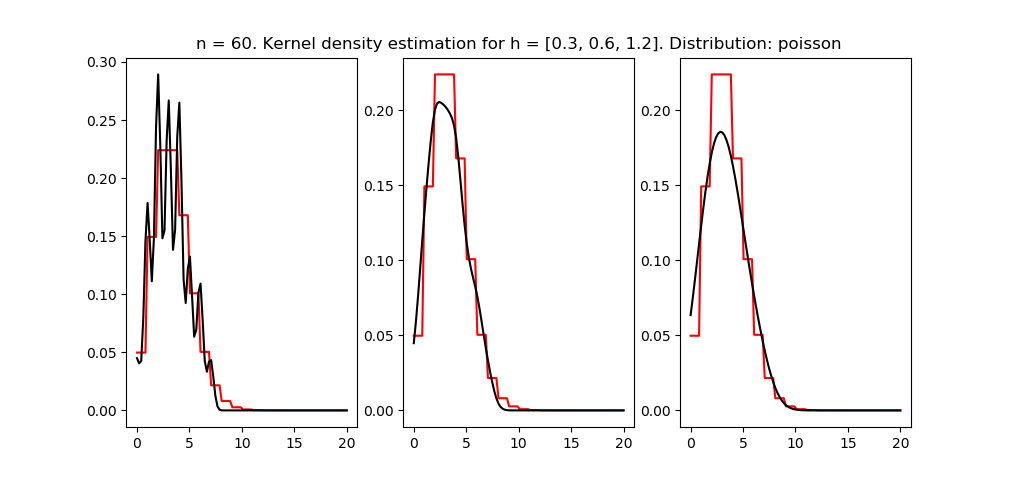
\includegraphics[width=\textwidth]{d_poisson60.png}
\end{figure}
    \begin{figure}[H]
 \caption{Ядерная функция плотности для распределения Пуассона \eqref{eqn:poisson}, n = 100}
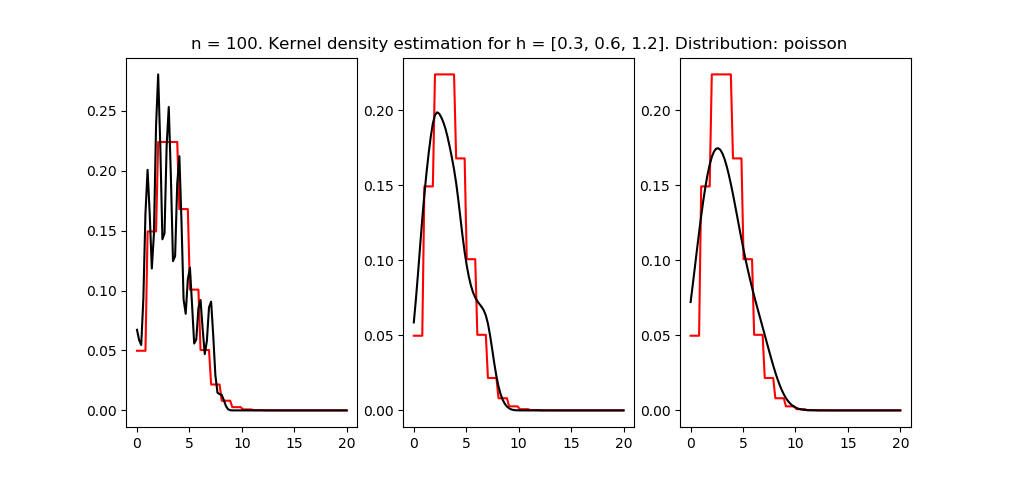
\includegraphics[width=\textwidth]{d_poisson100.png}
\end{figure}

    \begin{figure}[H]
 \caption{Ядерная функция плотности для равномерного распределения \eqref{eqn:uniform}, n = 20}
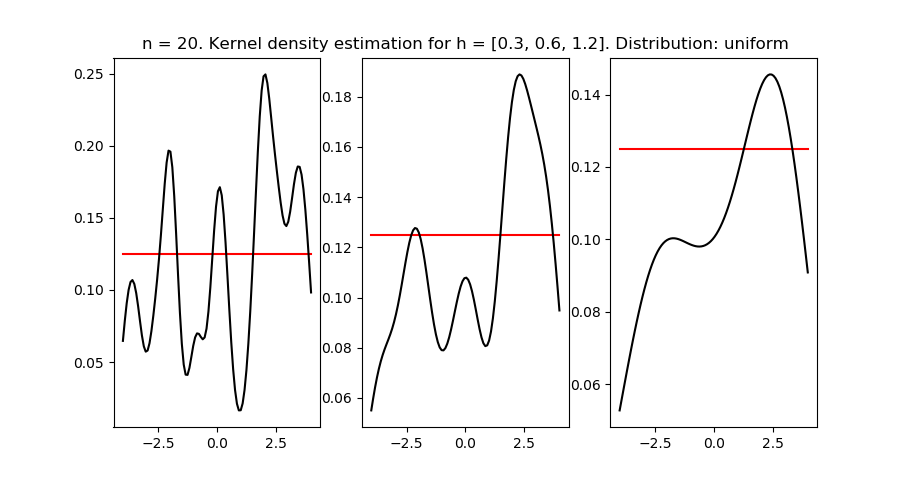
\includegraphics[width=\textwidth]{d_uniform20.png}
\end{figure}
    \begin{figure}[H]
 \caption{Ядерная функция плотности для равномерного распределения \eqref{eqn:uniform}, n = 60}
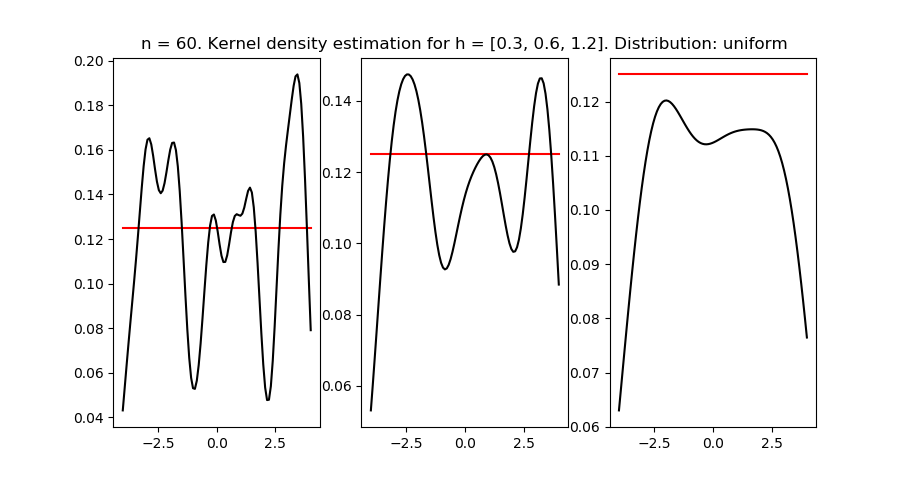
\includegraphics[width=\textwidth]{d_uniform60.png}
\end{figure}
    \begin{figure}[H]
 \caption{Ядерная функция плотности для равномерного распределения \eqref{eqn:uniform}, n = 100}
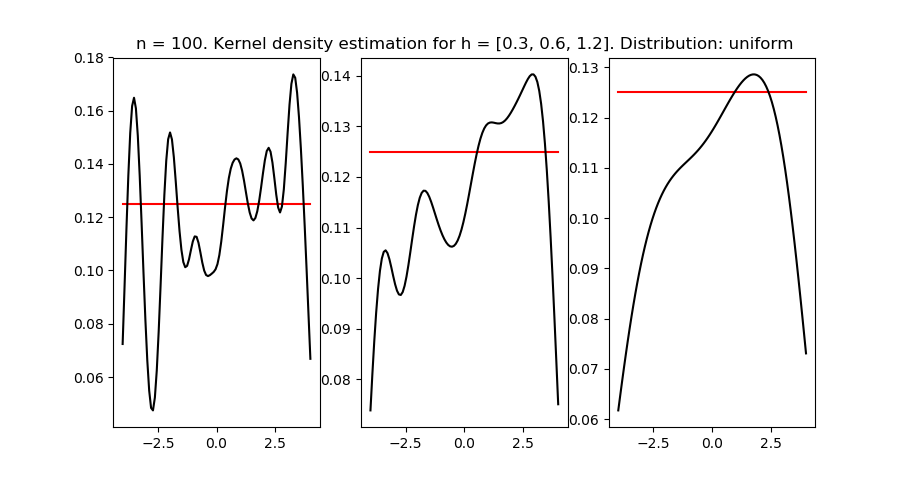
\includegraphics[width=\textwidth]{d_uniform100.png}
\end{figure}
\end{center}
\section{Обсуждение}
\subsection{Характеристики положения}
\par При вычислении средних значений пришлось отбрасывать некоторое число знаков после запятой, так как получаемая дисперсия не могла гарантировать получаемое точное значение. \par Иными словами дисперсия может гарантировать порядок точности среднего значения только до первого значащего знака после запятой в дисперсии включительно. \par Единственным исключением [в отбрасывании знаков после запятой] стало стандартное распределение Коши, так как оно имеет бесконечную дисперсию, а значит не может гарантировать никакой точности.

\section{Выводы}

\subsection{Плотности распределения вероятностей}
\par Как видно из графиков \eqref{fig:dis_norm_gis}, \eqref{fig:dis_lapl_gis}, \eqref{fig:dis_cauc_gis}, \eqref{fig:dis_pois_gis}, \eqref{fig:dis_uni_gis}, при увеличении размера выборки построенная гистограмма точнее приближает график соответствующего распределения.

\subsection{Характеристики положения}
\par В процессе работы вычислены значения характеристик положения для определённых распределений на выборках фиксированной мощности и получено следующее ранжирование характеристик положения:

\begin{enumerate}
    \item Стандартное нормальное распределение $$\overline{x} < Z_{tr} < Z_Q < med\;x < Z_R$$
    
    \item Стандартное распределение Коши $$med\;x < Z_Q < Z_{tr} < \overline{x} < Z_R$$
    
    \item Распределение Лапласа (коэффициент масштаба $\sqrt{2}$ коэффициент сдвига равен нулю) $$med\;x < Z_{tr} < \overline{x} < Z_Q < Z_R$$
    
    \item Равномерное распределение на отрезке $\left[-\sqrt{3},\sqrt{3}\right]$ $$Z_R < \overline{x} < Z_{tr} < Z_Q < med\;x$$
    
    \item Распределение Пуассона (значение мат ожидания равно $3$) $$\overline{x} < Z_{tr} < Z_Q < med\;x < Z_R$$
    
\end{enumerate}

\subsection{Боксплот Тьюки}
\par Экспериментально полученные проценты выбросок, близки к теоретическим
Можно вывести соотношение между процентами выбросов:

\begin{equation}
uniform<normal<poisson<laplace<cauchy
\end{equation}

\subsection{Эмпирические функции и ядерные оценки}
Эмпирическая функция лучше приближает эталонную функцию на больших выборках.

По визуальной оценке, наилучшее приближение функции распределения ядерной функции получено при увеличении ширины окна. При фиксированной ширине окна точнее приблизить функцию распределения позволяет увеличение выборки.


\begin{thebibliography}{}

     \bibitem{numpy}  Модуль numpy  -  https://physics.susu.ru/vorontsov/language/numpy.html
    
    \bibitem{distr_formulas}  
    Формулы распределений  -  https://vk.com/doc184549949\_491827451
    
    \bibitem{average}  
    Выборочное среднее  -  https://en.wikipedia.org/wiki/Sample\_mean\_and\_covariance
    
    \bibitem{med}  
    Выборочная медиана  -  http://femto.com.ua/articles/part\_1/2194.html
    
    \bibitem{mean_extr}  
    Полусумма экстремальных значений  -  https://studopedia.info/8-56888.html
    
    \bibitem{quartiles}  
    Квартили  -  https://studfiles.net/preview/2438125/page:13/
    
    \bibitem{cut_mean}  Усечённое среднее  -  https://ole-olesko.livejournal.com/15773.html
    
    
    
    \bibitem{med}  
    Выборочная медиана  -  http://femto.com.ua/articles/part\_1/2194.html
    
    \bibitem{quart}  
    Квартили -  https://studfiles.net/preview/2438125/page:13/
    
    \bibitem{sas} 
    Боксплот - https://en.wikipedia.org/wiki/Box\_plot
    
    
    
    
    
    \bibitem{plotlib} 
    Модуль matplotlib - https://matplotlib.org/users/index.html
    
    \bibitem{skp}
    Модуль scipy - https://docs.scipy.org/doc/scipy/reference/
    
    \bibitem{distr_formulas}  
    Формулы распределений  -  https://vk.com/doc184549949\_491827451
    
    \bibitem{emp}  
    Н. И. Чернова, https://nsu.ru/mmf/tvims/chernova/ms/lec/node4.html, 2002
    
    \bibitem{art}
    Victor, https://www.mql5.com/ru/articles/396, 2012
    
    \bibitem{link:pdf}
    Nathaniel E. Helwig, http://users.stat.umn.edu/\~helwig/notes/den-Notes.pdf, 2017

    
    
\end{thebibliography}


\end{document}
